\begin{figure}[ht!]  % 'htbp' suggests placement options
    \centering
    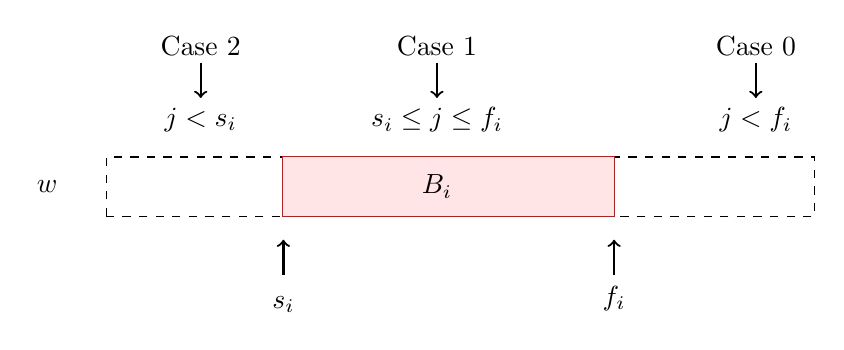
\begin{tikzpicture}[scale=1.5]
        % Main Rectangle w
        \draw[dashed] (0,0) rectangle (6,0.5);
        \node at (-0.5, 0.25) {\(w\)};

        % Smaller Rectangle 1 - Border color red
        \draw[draw=red, thick] (1.5,0) rectangle (4.3,0.5);
        
        \draw[->, thick] (1.5,-0.5) -- (1.5,-0.2);
        \node[align=center, below] at (1.5,-0.6) {\(s_{i}\)};
        \fill[red!10] (1.5,0) rectangle (4.3,0.5);
        \node at (2.8,0.25) {$B_{i}$};
        
        \draw[->, thick] (4.3,-0.5) -- (4.3,-0.2);
        
        \node at (4.3,-0.7) {$f_i$};
        
        
        \draw[->, thick] (5.5,1.3) -- (5.5,1);        
        \node[align=center, below] at (5.5,1) {\( j<f_i\)};
        \node[align=center, below] at (5.5,1.6) { \text{Case 0}};

        \draw[->, thick] (2.8,1.3) -- (2.8,1);        
        \node[align=center, below] at (2.8,1) {\( s_i \leq j \leq f_i\)};
        \node[align=center, below] at (2.8,1.6) {\text{Case 1}};

        \draw[->, thick] (0.8,1.3) -- (0.8,1);        
        \node[align=center, below] at (0.8,1) {\( j<s_i\)};
        \node[align=center, below] at (0.8,1.6) {\text{Case 2}};
        


    \end{tikzpicture}
    \caption{Compression for $w$ where $j$ is located.}
    \label{fig:case0}
\end{figure}